\documentclass[../report.tex]{subfiles}
\begin{document}	

% Introduction (A way of representing - KTH Lecture)
% --------------------------------------------------
% A. Known/Background
%    1. General
%    2. Specific problem
% B. Unknown problem (Where is the hole?)
% C. Research Purpose (Question you are going to answer)
% D. Experimental approach (What the question is and how are you going to address it?)
% Explain briefly about the scope of the problem
	
\chapter{Introduction} 
	\section{Bla bla}
Communication and collective thinking are the key to the development of human civilization. This development is driven by data - “The new oil of this digital era”. With the rise of media streaming services, there has been a huge surge in data traffic all over the world. It has also been estimated that by 2020 there will be 38.5 billion connected \gls{iot} devices \cite{gartner_iot,juniper_iot}.Here is another reference for example \cite{green_efficient_2001}

\begin{figure}[h]
	\centering
	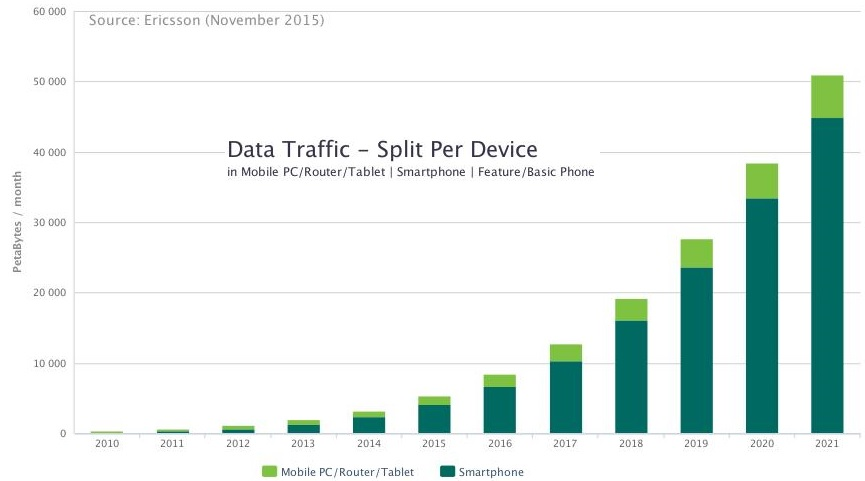
\includegraphics[width=1\textwidth]{1-data-traffic-forecast}
	\caption{Data traffic growth forecast to 2021, as per Ericsson, generated using }
	\label{fig:1_data_traffic_forecast}
\end{figure}



%\begin{itemize}
%	\item[$\square$] \textbf{Greater bandwidth}: Fiber provides more bandwidth than copper and can transmit up to 100 Gbps and beyond.
%	\item[$\square$] \textbf{Reliability and Immunity}: Fiber provides extremely reliable data transmission. It’s completely immune to many environmental factors that affect copper cable such as, electromagnetic and radio-frequency interference, crosstalk and impedance problems.  
%	\item[$\square$] \textbf{Security}: Fiber doesn’t radiate signals and is extremely difficult to tap, which provides better security than copper cables.
%	\item[$\square$] \textbf{Less attenuation}: Fiber optic transmission results in less attenuation (losses) than copper cables.
%	\item[$\square$] \textbf{Lightweight}: Fiber is lightweight, thin, and more durable than copper cable and takes up less space in cable trays.
%\end{itemize}

	\section{Bla bla}
%The performance of optical fiber networks is remarkable and it is this backbone which gives us a great user experience. The current internet architecture has already pushed the optical fiber to the network edges and the trend is to push it as close to the processor as possible. This has already opened up a new trend of “siliconizing photonics” \cite{silicon_photonics}, which arose from the research in microelectronics and photonics industry.\par 
%The electronics industry has pushed the boundaries of processing power of \gls{ic} by adding more transistors, according to Moore’s Law. Until recently, the increase in the speed, efficiency, and processing power of conventional electronic devices were achieved largely through clustering and downscaling of components on a chip. However, this trend toward miniaturization has yielded unwanted effects in the form of significant increases in noise, power consumption, signal propagation delay and aggravates already to serious thermal management problems. As a result, traditional microelectronics will soon fall short of meeting market needs, inhibited by the thermal and bandwidth bottlenecks inherent in copper wiring. Comparison in between Intel's processor speed and bus speed shows that although we have achieved good processing speed, the interconnects always find difficulty in catching up with the processing speed \cite{intel_proc_compare}. Annual global data center IP traffic will reach 10.4 zettabytes (863 exabytes per month) by the end of 2019, up from 3.4 zettabytes per year (287 exabytes per month) in 2014 \cite{cisco_forecast_2019}. Think of a server rack in a data center processing an average of this huge data per second, where interconnects between multiple processors in the server rack add up to a significant bottleneck. These bottlenecks can be overcome by substituting copper with optical interconnects, which can also operate at lower power and better efficiency. Additionally, optical interconnects can also improve switching and transmission of electrical signals as well as reduce heat dissipation.\par

	\section{Motivation for this thesis} 
%The dynamic control of optical polarization rotation can be utilized to realize a new class of components in integrated photonics including polarization mode modulators, multiplexers, filters, and switches for advanced optical signal processing, coherent communications, and sensing. Advanced sensors can be designed since more spectrometric analysis can be done using tunable modes. Furthermore, the concept can be useful in situations where polarization tuning is necessary under adiabatic conditions; for example in photon entanglement, which promises the development of even smaller micro-electronic devices along with secure communication channels. Moreover, since the power consumption of the \gls{tpr} is very low, this can be used for reconfiguration of network topology at low power. \par



	\section{Objectives of the thesis}
\textbf{Main objective}: To design and fabricate a low power TPS based on MEMS tuning. \\

\noindent \textbf{Sub objectives}: The areas which will be addressed are:
\begin{itemize}	
	\item[$\square$] Evaluate feasibility of . 
	\item[$\square$] Design a capable of tuning polarization in between the two fundamental waveguide modes.
	\item[$\square$] Demonstration of the  with an extinction ratio of more than at least \SI{10}{\decibel} for the two fundamental modes, in C and L bands.
\end{itemize}
	
	\section{Outline of this thesis}
%The outline of the thesis is as follows: Background, motivation and the research questions being addressed, is discussed in Chapter 1. Background literature of optical waveguide theory is discussed in Chapter 2. In Chapter 3, the current state of art for the available passive and active \gls{pr} solutions are discussed. Here, also the working principle of the current available designs are explained along with the areas which can be improved. Chapter 4 discusses the design of the final system and the simulation results obtained. In Chapter 5, the fabrication details are provided along with the \gls{sem} images of the fabricated product. Experiments and results are discussed in Chapter 6. In Chapter 7, the known limitations of the designed \gls{tpr} are discussed along with future optimizations and work possibilities. Finally, the thesis is concluded with ending remarks in Chapter 8.
	
\end{document}
